%\section {Définitions}

%
%  Robot
%

\begin{frame} {Articulations}
  \centerline {
    \parbox {.53\linewidth} {
      \emph{Robot}~: Ensemble de corps rigides li\'ees les uns aux autres par des \textit{articulations}.
      \vskip .5cm
      \pause
      \emph{Transformation}~: une translation $\trans$ et une rotation $\rotation$.
      L'ensemble des transformations forment l'espace $SE(3)$.
      \vskip .5cm
      \pause
      \emph{Articulation}~: transformation $\left( \trans(\conf), \rotation(\conf) \right)$ entre deux repères param\'etr\'es par une ou plusieurs
      variables $\conf \in \real^n$.
    }
    \parbox{.45\linewidth} {
      \centerline {
        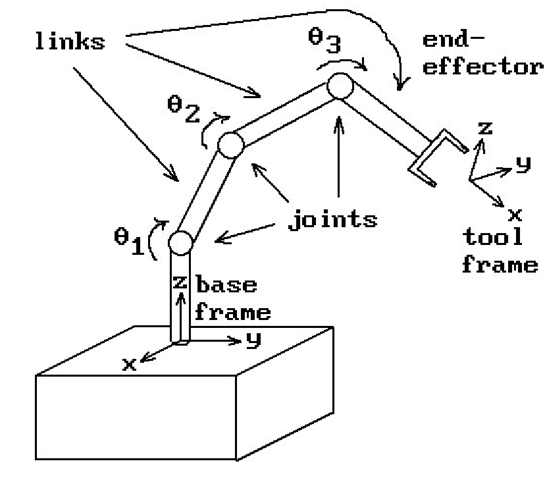
\includegraphics[width=\linewidth]{img/kinematic_chain.png}
      }
    }
  }
\end{frame}

%
%  Articulation
%
\begin{frame} {Articulations: Rotation 1D}
  \centerline {
    \parbox {.53\linewidth} {
      \begin {itemize}
      \item Rotation autour de \z~:
        \begin{eqnarray*}
          \real & \rightarrow & SE(3) \\
          \conf_0 & \rightarrow & (0_{\real^3}, \rotation)
        \end{eqnarray*}
      \end {itemize}
      \vskip .5cm
      \pause
      $$ \rotation=\left(\begin{array}{ccc}\cos \conf_0 & -\sin \conf_0 & 0 \\ \sin \conf_0 & \cos \conf_0 & 0 \\ 0&0&1\end{array}\right)$$
    }
    \parbox{.45\linewidth} {
      \centerline {
        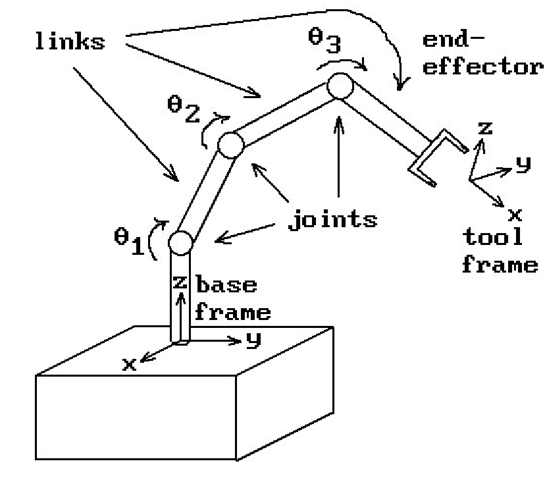
\includegraphics[width=\linewidth]{img/kinematic_chain.png}
      }
    }
  }
\end{frame}

%
%  Articulation
%
\begin{frame} {Articulations: Translation 1D}
  \centerline {
    \parbox {.53\linewidth} {
      \begin {itemize}
      \item Translation selon \x~:
        \begin{eqnarray*}
          \real & \rightarrow & SE(3) \\
          \conf_0 & \rightarrow & (\trans, I_3)
        \end{eqnarray*}
      \end {itemize}
      \vskip .5cm
      \pause
      $$ \trans=\left(\begin{array}{c} \conf_0 \\ 0 \\ 0 \\ \end{array}\right)$$
      $$ I_3=\left(\begin{array}{ccc} 1 & 0 & 0 \\ 0 & 1 & 0 \\ 0&0&1\end{array}\right)$$
    }
    \parbox{.45\linewidth} {
      \centerline {
        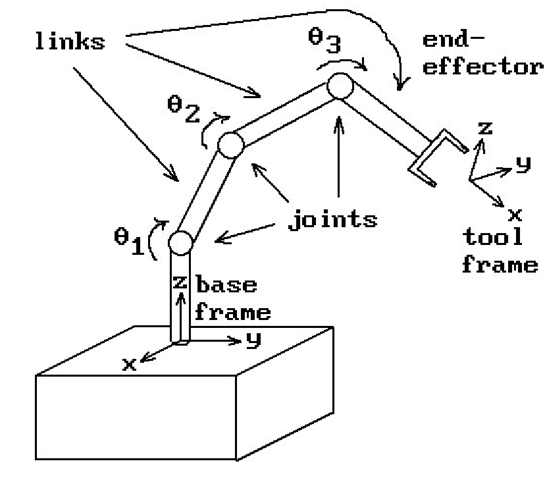
\includegraphics[width=\linewidth]{img/kinematic_chain.png}
      }
    }
  }
\end{frame}

%
%  Articulation
%
\begin{frame} {Articulations: Translation 3D}
  \centerline {
    \parbox {.53\linewidth} {
      \begin {itemize}
      \item Translation~:
        \begin{eqnarray*}
          \real^3 & \rightarrow & SE(3) \\
          \left( \conf_0,\conf_1,\conf_2 \right) & \rightarrow & (\trans, I_3)
        \end{eqnarray*}
      \end {itemize}
      \vskip .5cm
      \pause
      $$ \trans=\left(\begin{array}{c} \conf_0 \\ \conf_1 \\ \conf_2 \\ \end{array}\right)$$
      $$ I_3=\left(\begin{array}{ccc} 1 & 0 & 0 \\ 0 & 1 & 0 \\ 0&0&1\end{array}\right)$$
    }
    \parbox{.45\linewidth} {
      \centerline {
        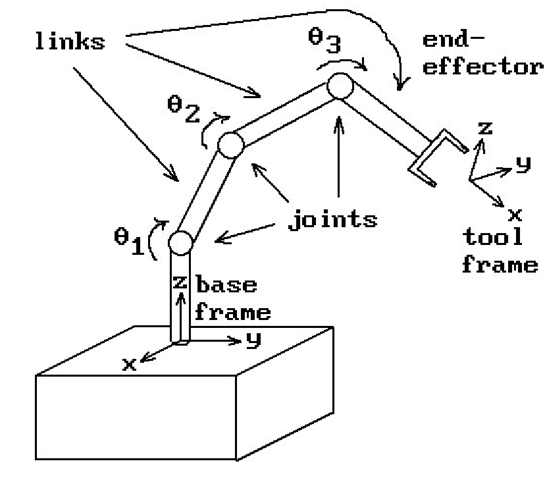
\includegraphics[width=\linewidth]{img/kinematic_chain.png}
      }
    }
  }
\end{frame}

%
%  Articulation
%
\begin{frame} {Articulations: Rotation 3D}
  \centerline {
    \parbox {.54\linewidth} {
      \begin {itemize}
      \item Vecteur de taille 4 unitaire:
        $$\mathbb{S}^4 = \left\{ \conf | \conf\in\real^4, ||\conf||=1 \right\}$$
      \pause
      \item Rotation~:
        \begin{eqnarray*}
           \mathbb{S}^4 & \rightarrow & SE(3) \\
           \conf & \rightarrow & (0_{\real^3}, \rotation(\conf))
        \end{eqnarray*}
      \end {itemize}
      \vskip .5cm
      \pause
      {\tiny
          $$\begin{array}{c}R(\conf)=\\
          \left(\begin{array}{ccc}1 - 2(\conf_2^2 + \conf_3^2) & 2\conf_2\conf_1 - 2\conf_3\conf_0 & 2\conf_3\conf_1 + 2\conf_2\conf_0\\ 2\conf_2\conf_1 + 2\conf_3\conf_0 & 1 - 2(\conf_1^2 + \conf_3^2) & 2\conf_3\conf_2 - 2\conf_1\conf_0\\ 2\conf_3\conf_1 - 2\conf_2\conf_0 & 2\conf_3\conf_2 + 2\conf_1\conf_0 & 1 - 2(\conf_1^2 + \conf_2^2)\end{array}\right)\end{array}$$
          $$\conf_0 + \conf_1 i + \conf_2 j + \conf_3 k\ \mbox{is a quaternion.}$$
      }
    }
    \parbox{.45\linewidth} {
      \centerline {
        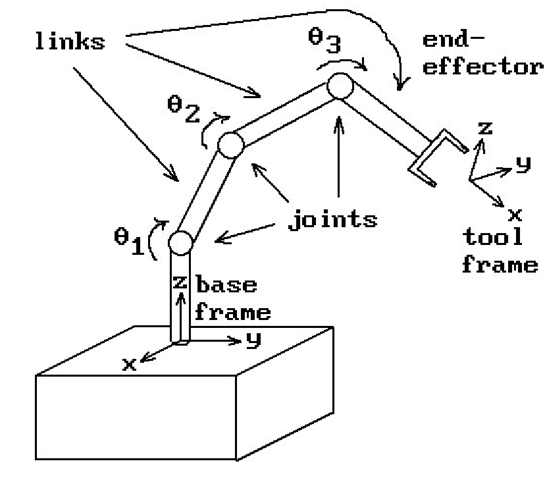
\includegraphics[width=\linewidth]{img/kinematic_chain.png}
      }
    }
  }
\end{frame}

%
%  Quaternions
%
\begin{frame} {Digression: Quaternions}
  \begin{itemize}
    \item Nombres complexes: $i^2 = -1$
    \item Quaternion: extension des nombres complexes
      $$i^2 = j^2 = k^2 = ijk = -1$$
      d'o\`u l'on d\'eduit
      $$ ij=k,\ jk=i,\ ki=j$$
    \item $\conf = \conf_3 + \conf_0 i + \conf_1 j + \conf_2 k $, with $\conf\in\real^4$.
    \item Quaternion unitaire: $\conf_3^2 + \conf_0^2  + \conf_1^2 + \conf_2^2  = 1$.
  \end{itemize}
\end{frame}

%
%  Quaternions
%
\begin{frame} {Digression: Rotation 3D et quaternion unitaire}
  \centerline {
    \parbox{.30\linewidth} {
      \centerline {
        \graphicspath{{./img/}}
        \def\svgwidth{\linewidth}
        \input{img/Angle_axis_vector.pdf_tex}
      }
    }
    \parbox {.68\linewidth} {
      \begin {itemize}
        \item<1-> Rotation identit\'e: $ \conf = \left( 0, 0, 0, 1 \right)$
        \item<2-> Rotation de $\theta$ autour de $\vect{e}$
          $$ \conf = \left( \vect{u}_0, \vect{u}_1, \vect{u}_2, cos(\frac{\theta}{2}) \right)$$
          avec $ \vect{u} = sin(\frac{\theta}{2}) \vect{e}$.
        \item<3->$\conf$ et $-\conf$ repr\'esente la m\^eme rotation.
      \end {itemize}
    }
  }
\end{frame}

%
%  Chaine cinematique
%
\begin{frame} {Cha\^ine cin\'ematique}
  \centerline {
    \parbox {.59\linewidth} {
      \begin {itemize}
        \item Sequence de 3 rotations : $\M{1}{1'}(\conf_1)$,
          $\M{2}{2'}(\conf_2)$ et $\M{3}{3'}(\conf_3)$.
        \item Articulation rigidement li\'ee entre elles : $\M{0}{1}$,
          $\M{1'}{2}$, $\M{2'}{2}$ et $\M{3'}{outil}$.
        \item Configuration du robot: $\conf = \left( \conf_1, \conf_2, \conf_3 \right)$
        \item Calcul de la position de l'outil :
      \end {itemize}
    }
    \parbox{.40\linewidth} {
      \centerline {
        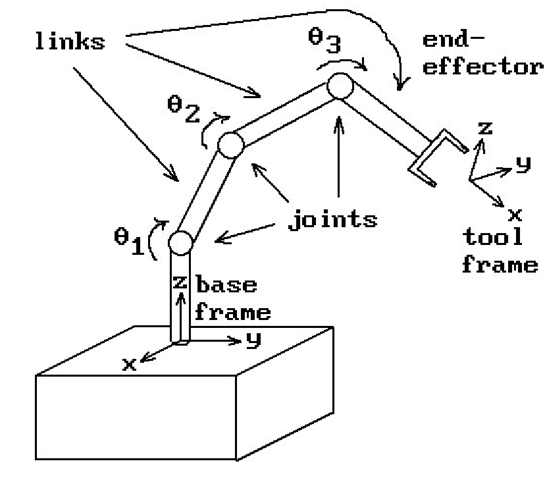
\includegraphics[width=\linewidth]{img/kinematic_chain.png}
      }
    }
  }
  $$
  \M{0}{outil} =
  \M{0}{1}           .
  \M{1}{1'}(\conf_1) .
  \M{1'}{2}          .
  \M{2}{2'}(\conf_2) .
  \M{2'}{3}          .
  \M{3}{3'}(\conf_3) .
  \M{3'}{outil}
  $$
\end{frame}

%
%  Jacobienne
%
\begin{frame} {Cha\^ine cin\'ematique : Jacobienne}
  \centerline {
    \parbox {.59\linewidth} {
      \begin{itemize}
        \item<1-> Contr\^ole du robot via les moteurs: $\conf$
        \item<2-> On veut contr\^oler l'organe terminal: $\M{0}{outil}$
        \item<3-> Relation entre $\dot{\conf}$ et $\vect{V}_{A\in outil / 0}$ ?
        \item<4-> Relation entre $\tau$        et $\vect{F}_{A, outil / 0}$ ?
      \end{itemize}
    }
    \parbox{.40\linewidth} {
      \centerline {
        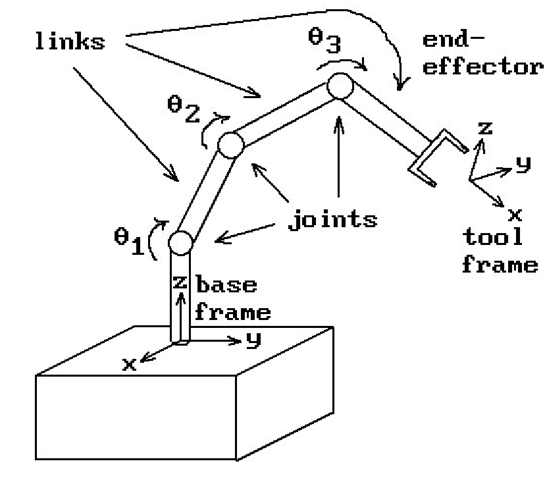
\includegraphics[width=\linewidth]{img/kinematic_chain.png}
      }
    }
  }
\end{frame}

%%%%%%%%%%%%%%%%%%%%%%%%%%%%%%%%%%%%%%%%%%%%%%%%%%%%%%%%%%%%%%%%%%%%%

\begin{frame} {Un cas plus complexe: robot humano\"ide}
  \centerline {
    \parbox{.66\linewidth} {
      Cha\^ine cin\'ematique:
      \vskip .5cm
      \centerline {
        \def\svgwidth {.5\linewidth}
        {\tiny
          \graphicspath{{./figures/}}
          \input {figures/kinematic-chain.pdf_tex}
        }
      }
      \vskip .5cm
      N\'ec\'essit\'e de repr\'esenter un corps flottant.
    }
    \parbox {.33\linewidth} {
      \centerline {
        \includegraphics[width=\linewidth]{figures/hrp2.jpg}
      }
    }
  }
\end{frame}

%
%  Obstacle
%

\begin{frame} {Definitions}

\begin{itemize}
  \item \emph{Espace de travail} dans lequel le robot bouge: $\WS=\real^2$ o\`u $\real^3$
    \pause
  \item Obstacle dans $\WS$: sous-ensemble compact de $\WS$, not\'e $\obst$.
    \pause
  \item Espace des configurations: $\CS$.
    \pause
  \item Position en une configuration $\conf$ d'un point $M\in\body_i$:
    $\x_i(M,\conf)$.
    \pause
  \item Obstacle dans l'espaces des configurations:
    \begin{eqnarray*}
      \CSobst&=\{\conf\in\CS,&\exists i\in\{1,\cdots,m\},\ \exists M\in\body_i,\ \x_i(M,\conf)\in\obst\ \mbox{or}\\
      &&\exists i,j\in\{1,\cdots,m\},\ \exists M_i\in\body_i,\ \exists M_j\in\body_j,\\
    &&\x_i(M_i,\conf)=x_j(M_j,\conf)\}
  \end{eqnarray*}
  \pause
\item Espace des configurations \emph{libres}: $\CSfree = \CS\setminus\CSobst$.
\end{itemize}
\end{frame}

%
%  Motion
%

\begin{frame} {Chemin}
  \begin{itemize}
    \item Chemin:
      \begin{itemize}
        \item fonction continue de $[0,1]$ dans $\CS$.
      \end{itemize}
      \pause
    \item Chemin sans collision:
      \begin{itemize}
        \item fonction continue de $[0,1]$ dans $\CSfree$.
      \end{itemize}
  \end{itemize}
\end{frame}

%
%  Motion
%

\begin{frame}{Probl\'eme de planification de mouvement}
  \begin{itemize}
    \item \'Etant donn\'e un robot, des obstacles ainsi qu'une configuration initial et finale du robot,
      \begin{itemize}
        \item<2-> trouver un chemin sans collision allant de la configuration initiale à la configuration finale.
      \end{itemize}
  \end{itemize}
  \onslide+<3->{
    \begin{itemize}
      \item \'Etant donn\'e un robot, $\obst$, $(\conf_{initiale}, \conf_{finale})\in\CS^2$,
        \begin{itemize}
          \item \onslide+<4-> {trouver $f\in\mathcal{C}^0([0,1], \CSfree)$ telle que $f(0) = \conf_{initiale}$ et $f(1) = \conf_{finale}$.}
        \end{itemize}
    \end{itemize}
  }
\end{frame}
